\documentclass[prb,preprint]{revtex4-1} 


\usepackage{amsmath}  
\usepackage{amsfonts} 
\usepackage{graphicx} 
\usepackage{color}
\usepackage{ulem}

\begin{document}


\title{Recreating Young's Double Slit Experiment}


\author{Edward Lipchus}
\email{ejl13@hampshire.edu}
\affiliation{Department of Natural Science, Hampshire College, Amherst, MA 01002}


\author{Danika Luntz-Martin}
\email{dluntzma@smith.edu}
\affiliation{Department of Physics, Smith College, Northampton, MA 01063}


\date{\today}



\begin{abstract}

In 1803, Young performed his famous Double Slit Experiment to determine whether light acted as a particle or as a wave. Recreating his ground-breaking work, we observed the double slit interference pattern associated with light as a wave, and fit each of our three data sets using both the Fraunhofer and the Fresnel models - the former calculating the path of light strictly based on angle and the latter integrating over the entire path length of each light beam. Our models fit decently with reduced $\chi^2$ values of 73, 70, and 122 for the Fraunhofer and of 53, 54, and 122 for the Fresnel, and showed that the Fresnel model provided a better fit for our experimental set-up.

\end{abstract}

\maketitle 


\section{Introduction} 

Early scientists debated the nature of light,�� whether it was a particle or a wave. In 1803, Thomas Young performed an experiment to see if light acted as a wave or as a particle by passing a coherent light source through two closely spaced slits. If light was a particle, you would see to thin lines of illumination in line with the slits, as the particles simply passed through the slits. If, however, light was a wave, then the two slits would act as the origins of two wave sources that could interfere with each other, constructively and destructively, and a corresponding pattern would emerge opposite the slits. These are depicted in Fig. \ref{PartVsWave}.

\begin{figure}[h!]
\centering
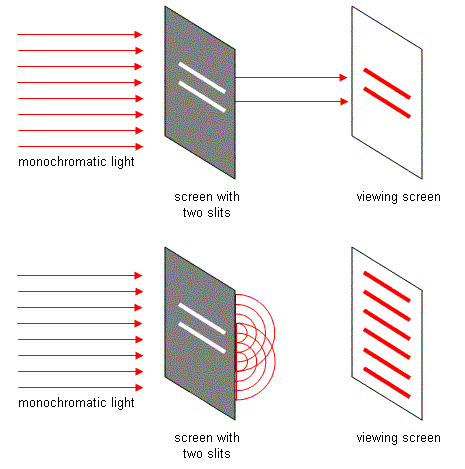
\includegraphics[width=6in]{DoubleSlitPicsStudyPhysicsCa.png}
\caption{Image of light passing through a double slit if it were a particle (above) and if it were a wave (below).\cite{studyphysics}}
\label{PartVsWave}
\end{figure}

The interference pattern is brightest in the center, getting fainter each step away from the center, as the two light waves interfere constructively to form peaks and destructively to leave empty valleys. The spacing between peaks is determined by the equation:
\begin{equation}
\label{DblIntfr}
x = \frac{n\lambda L}{d}\cite{studyphysics}
\end{equation}
Where x is the distance from the center, n is the peak number from the center – with $n=1$ being the peak on either side of the center line – $\lambda$ is the wavelength of the light, L is the distance from the double slit to the screen upon which the light is shining, and d is the spacing between the slits.

Young passed sunlight through a single slit – making it a single line of coherent light – before letting it pass through a double slit and then onto a projection screen, upon which he saw an interference pattern. Light was, undoubtedly, a wave.

There are two general ways to look at modeling this diffraction, based on a dimensionless number called the Fresnel Number.\cite{Wolfram} This number is defined as:
\begin{equation}
\label{DblIntfr}
F = \frac{a^2}{\lambda R}
\end{equation}
Where $a$ is the size of the slit, $\lambda$ is the wavelength of the incident light, and $R$ is the distance from the slit to the detection screen. If this number is very much less than one (by having the detection screen be far away from the slit, for instance), then it is reasonable to take the Fraunhofer limit for diffraction, which effectively ignores the distance to the screen and relies only on the angle between the slit and the screen.\cite{Wolfram} On the other hand, when the Fresnel number is greater than or equal to one, the Fresnel Diffraction model must be used, which takes into account path lengths traveled by the light.\cite{Wolfram} 

\section{Methods}

We used the TeachSpin Two-Slit Interference, One Photon at a Time (TWS1-B) which is a apparatus designed to perform Young's double slit experiment. The apparatus has two light sources, a 670 nm diode laser and a light bulb with a removable green light filter. There are four slit holders spaced throughout the length of the apparatus, see Figure~\ref{apparatus}. The first slit, the source slit, eliminates excess light from the light source and approximates a plane wave. Next is the double slit, our double slit had 0.1mm wide slits and center-to-center separation of 0.353mm. Following the double slit was a wide single slit attached to a micrometer, called the slit blocker. The slit blocker could be moved to block either or both slits of the double slit. Finally there was a detector slit which allowed us to measure the intensity of light (using the laser) or the number of photons (using the light bulb) over a small region of the x-axis. The micrometer attached to the detector slit allowed us to scan along the x-axis. When we worked with the laser as our light source, we used the built in photodetector which gave an output voltage that was proportionate to the light intensity. When we used light bulb as our light source, we used the built in photo-multiplier tube (PMT) attached to the TeachSpin Pulse Counter / Interval Timer (PCIT1) to count the number of photons.


\begin{figure}[h!]
\centering
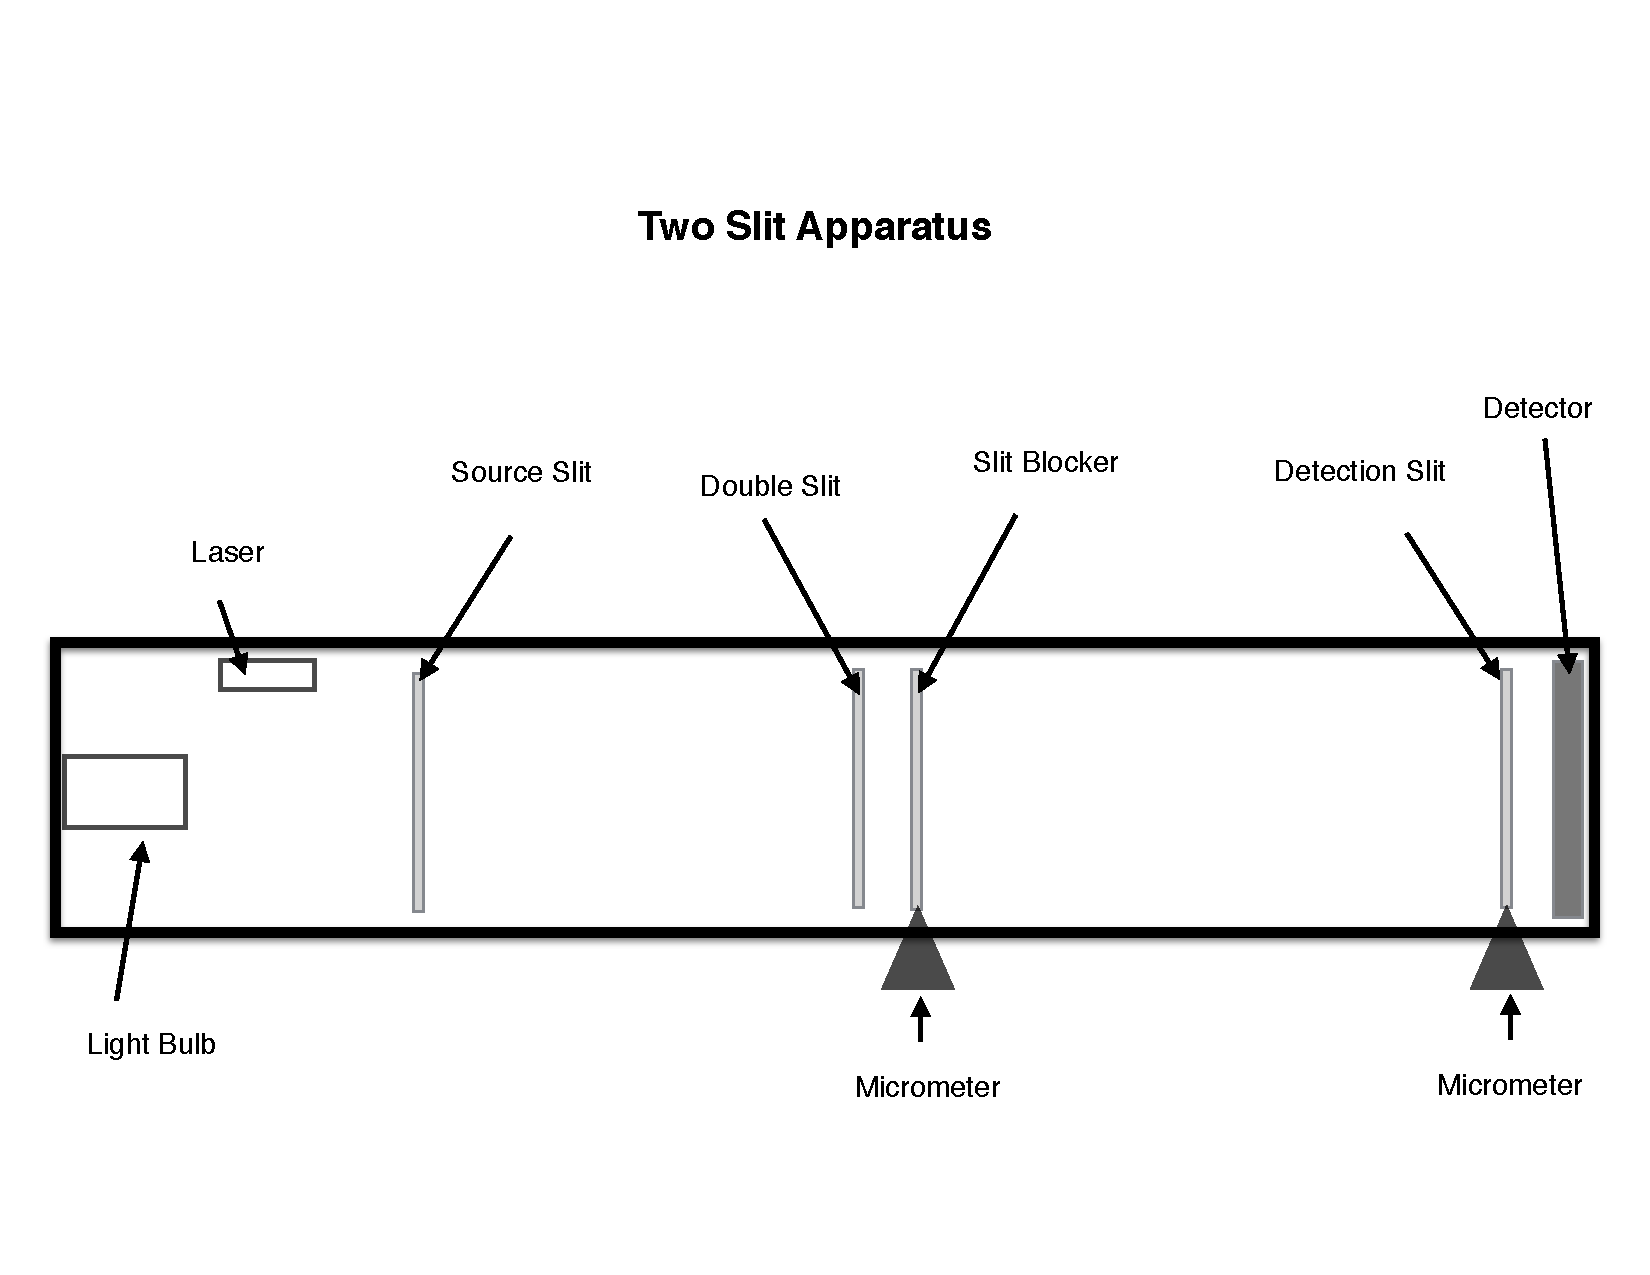
\includegraphics[width=6in]{apparatus.pdf}
\caption{The experimental set-up of the apparatus we used. The laser can slide into place in front of the light bulb. The source slit is a wide slit that blocks extraneous light from the light source. The slit blocker is another wide slit that can be moved, using the micrometer, to block one of the double slits, effectively turning it into a single slit. The detector slit allowed us to count the number of photons reaching the detector over a small region. The micrometer allowed us to scan across the detector and get a photon count at each x value.}
\label{apparatus}
\end{figure}


We began by aligning the slits within our apparatus. We started by using the laser roughly align the source slit and double slit and ensure that the double slit was not tilted. Then we made fine adjustments to the alignment using the light bulb. Throughout our experiments we used a midrange light bulb power setting of 5. We used a green filter on our light bulb to lower the intensity of the light and narrow the range of wavelengths to 541 - 551nm. 

Next we optimized the signal-to-noise ratio for our PMT. To do so we held the PMT voltage constant and varied the discriminator threshold. We found that dial value of the PMT voltage was not consistent with the measured value of the PMT voltage using a digital multimeter, so we used the multimeter reading to determine our voltage. For each value of the discriminator threshold we measured four values for our signal plus our noise and four values of just noise with no signal. We then averaged each set of four values and took the ratio to calculate the signal-to-noise. In our case the ratio we actually calculated was signal and noise to noise, this difference should scale our results but not change the overall outcome. The calculated signal-to-noise ratios can be seen for various PMT voltages in Figure~\ref{signaltonoise}. The highest values for the PMT voltage, 900 V and 800 V, had a significantly lower signal-to-noise ratio. The lower values for the PMT voltage, 600 V and 650 V, required small values for the discriminator threshold and did not have as high a signal-to-noise ratio. The highest signal-to-noise ratio we obtained was for PMT voltage of 750 V and a discriminator threshold of 15.

\begin{figure}[h!]
\centering
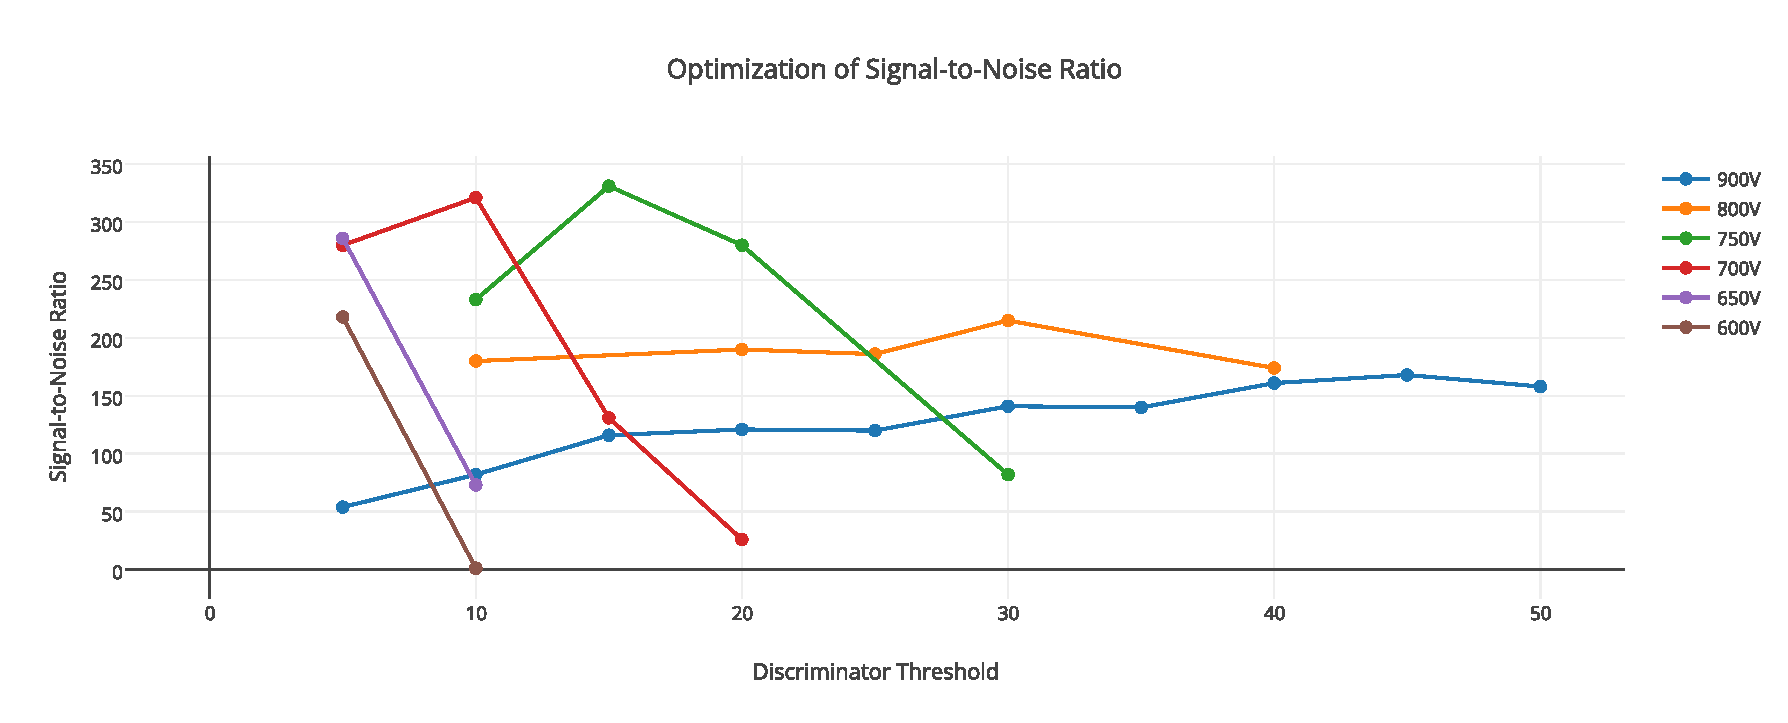
\includegraphics[width=6in]{signaltonoise.pdf}
\caption{The signal-to-noise ratios we obtained for a range of discriminator thresholds for various PMT voltages. For the high PMT voltages, 900 V (blue) and 800 V (orange) the signal-to-noise ratio was much lower. For lower PMT voltages, 650 V (purple) and 600 V (brown), the signal-to-noise ratio was again lower. The optimal signal-to-noise ratio was at a PMT voltage of 750 V (green) and a discriminator threshold value of 15.}
\label{signaltoniose}
\end{figure}

To collect data we used a Labview program called ``TeachSpin Counter V3'' that connected to the pulse counter. We then moved the detector slit along the x-axis in increments of 0.05 mm and recorded the number of counts given by the pulse counter. We were careful when collecting multiple sets of data to only scan along the x-axis in one direction and turn the micrometer father than necessary to minimize any backlash effects.

\section{Results}

We collected three sets of data using the double slit arrangement. Figure~\ref{doubleslit} shows a representative selection of the data we collected. The alignment of our slits was not exact because the minima at smaller x values do not reach zero. However, the vertical offset was not linear so it could not easily be subtracted off.

\begin{figure}[h!]
\centering
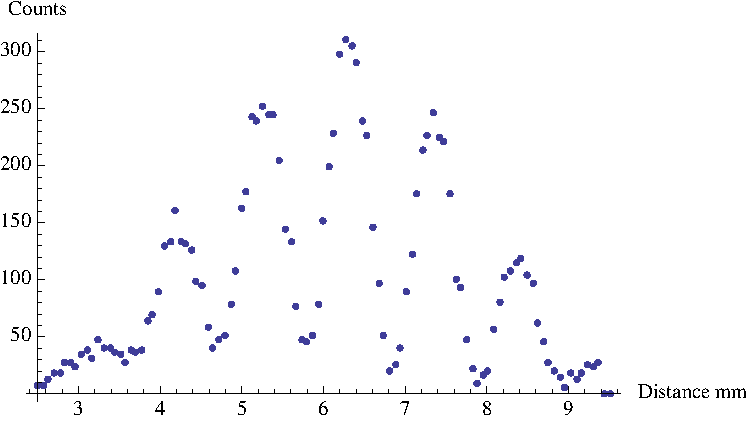
\includegraphics[width=6in]{doubleslit.pdf}
\caption{Data collected for the double slit arrangement. Our alignment was imperfect because the minima on the right side do not reach zero.}
\label{doubleslit}
\end{figure}

Using the slit blocker we were able to obtain single slit data from both the near and the far slits. We found further evidence of the misalignment of our slits. The intensity of the near slit, Figure~\ref{singlenear}, was one fourth of the intensity of the double slit arrangement which in is agreement with theory. However the intensity of the far slit, Figure~\ref{singlefar}, was twice the intensity of the near slit and nearly twice the intensity predicted by theory. The discrepancy was mostly likely caused by our inability to exactly align the slits. It is also possible that the increase in intensity was caused by a reflection off the wall the apparatus that was was going around the silt instead of through it.

\begin{figure}[h!]
\centering
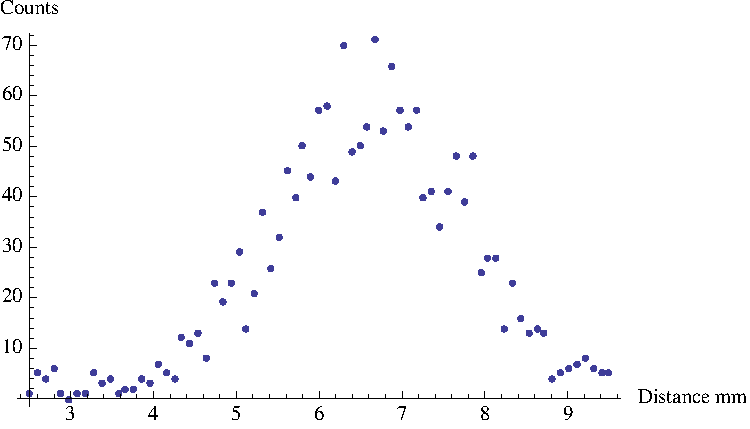
\includegraphics[width=6in]{singlenear.pdf}
\caption{Data collected for a single slit arrangement using the near slit. There appears to be a large uncertainty, note the wide band of data points. The intensity of the near single slit is approximately one fourth the intensity of the double slit.}
\label{singlenear}
\end{figure}

\begin{figure}[h!]
\centering
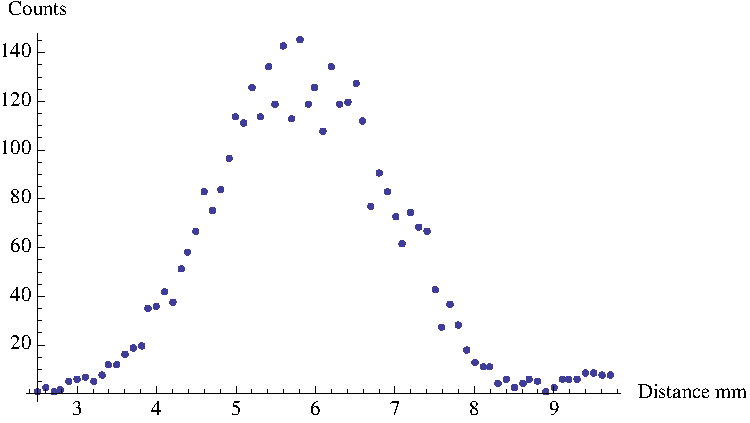
\includegraphics[width=6in]{singlefar.pdf}
\caption{Data collected for a single slit arrangement using the far slit. There is again a large uncertainty evident from the wide line of data points. The intensity of this slit is nearly twice the intensity of the near slit. This is mostly likely due to misalignment or reflected light from outside the slit.}
\label{singlefar}
\end{figure}


\section{Analysis}

The purpose of our experiment was to observe the quantum mechanical wave-like properties of a single photon. We wanted to see a diffraction pattern when only a single photon was passing through the slits which would suggest that the single photon was interfering with itself.

To make our results significant we need to show that there is only one photon in the apparatus at a time. The distance from the source slit to the detector slit is $88 \pm 1$ cm. Light travels at $2.998 \text{x} 10^{10}$ cm/s. So the time that a photon spends in the apparatus, $t = L/c$, is equal to $2.94 \pm 0.03$ ns. We collected data in one second periods. The most counts we got in a one second period was 350. That means that on a average one photon arrives at the detector every $2.86$ ms. There is only photons in the apparatus for $1029 \pm 10$ ns out of the second. That means that $99.9999\%$ of the time the apparatus is empty. The chances of there being more than one photon in the apparatus at a time are negligible. This means that the wave-like results we saw were cause by each photon interfering with itself.

We used two different models to fit to our double slit data, the Fraunhofer model and the Fresnel model. We did all of our data fitting in Mathematica and the code we used can be found in the appendix. Figures~\ref{doublefraun1}-\ref{doublefraun3} are our double slit data with fits using the Fraunhofer model. The $\chi^2$ and reduced $\chi^2$ values for both the Fraunhofer and Fresnel fits can be found in Table~\ref{chisquared}.

\begin{figure}[h!]
\centering
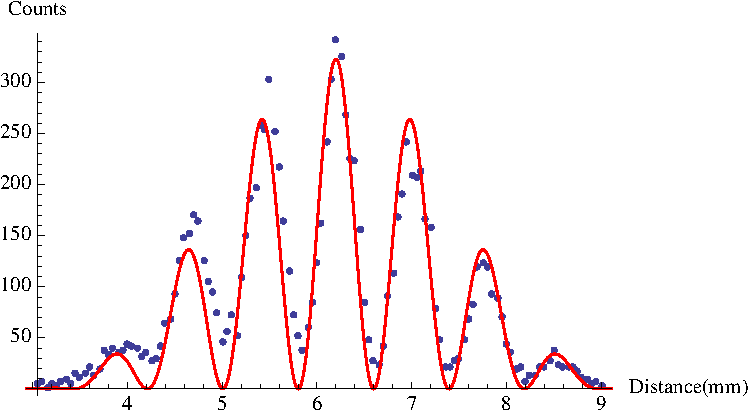
\includegraphics[width=6in]{doublefraun1.pdf}
\caption{Double slit data from our first run with a fit using the Fraunhofer model. The fit is much better on the right side than the left due to the alignment issues previously discussed.}
\label{doublefraun1}
\end{figure}

\begin{figure}[h!]
\centering
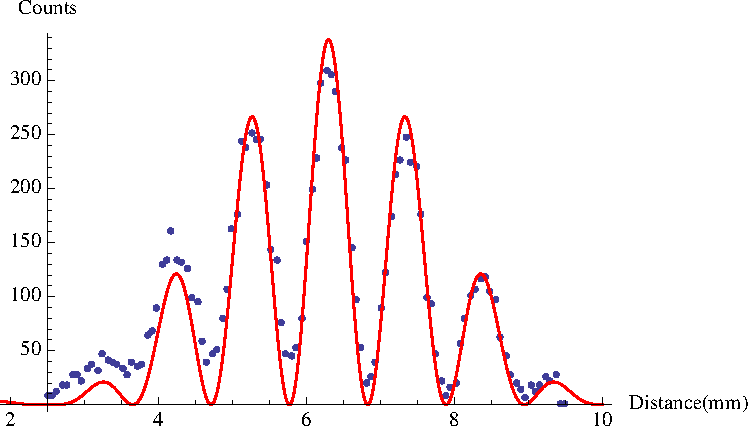
\includegraphics[width=6in]{doublefraun2.pdf}
\caption{Double slit data from our second run with a fit using the Fraunhofer model. The fit is again much better on the right side than the left due primarily to the misalignment.}
\label{doublefraun2}
\end{figure}

\begin{figure}[h!]
\centering
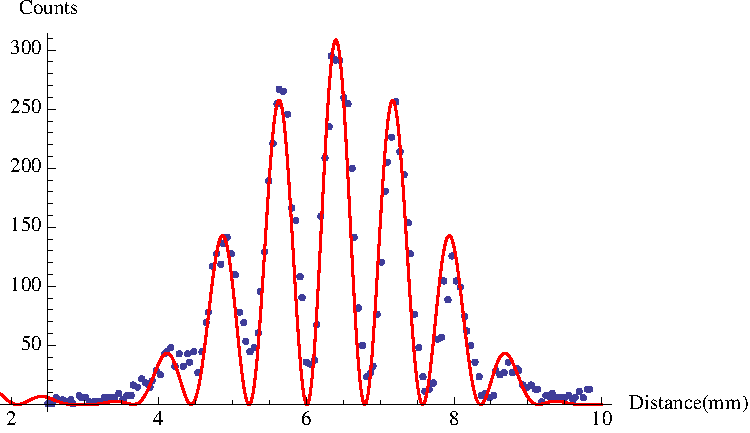
\includegraphics[width=6in]{doublefraun3.pdf}
\caption{Double slit data from our third run with a fit using the Fraunhofer model. This fit is slightly better on the left side than the right.}
\label{doublefraun3}
\end{figure}

The Fraunhofer model uses diffraction and assumes that the detection location is far away from the place of diffraction. For the double slit arrangement it gives the function

\begin{equation}
\label{fraunhofer}
I(x) = I_0 \left(\frac{\sin\alpha}{\alpha}\right)^2 \left(\cos\beta\right)^2
\end{equation}

were $I_0$ is the maximum intensity. $\alpha$ and $\beta$ are defined as

\begin{equation}
\label{alpha}
\alpha = \frac{a \pi \sin(\frac{x - x_0}{R})}{\lambda}
\end{equation}

\begin{equation}
\label{beta}
\beta = \frac{d \pi \sin(\frac{x - x_0}{R})}{\lambda}
\end{equation}

where $\lambda$ is the wavelength of the light, $a$ is the width of each slit, $d$ is the center-to-center slit separation and $R$ is the distance from the double slit to the detector. We defined $x$ to be the axis that we scanned along with the detector slit and $x_0$ is a fit parameter to adjust for the offset of the central peak.
Because the $\alpha$ contains a sine function, it can be zero. This causes problems since $\alpha$ is in the denominator of a fraction making Equation~\ref{fraunhofer} undefined. To avoid the undefined places in Equation~\ref{fraunhofer} we used a sinc function which is continuous and takes the limit as $\alpha$ approaches zero.

We also used the Fresnel model to fit all of our data. The Fresnel model sums over all of the possible paths that the photon could take. The functions for the Fresnel model are

\begin{equation}
\label{fresnelnear}
I_\text{near} = e^{\frac{2 \pi I D_1}{\lambda}} e^{\frac{2 \pi I D_2}{\lambda}} \int_\frac{d-a}{2}^\frac{d+a}{2} e^{\frac{2 \pi I (w-y_1)^2}{2 D_1 \lambda}} e^{\frac{2 \pi I (y_1-z)^2}{2 D_2 \lambda}} dy_1
\end{equation}

\begin{equation}
\label{fresnelfar}
I_\text{far} = e^{\frac{2 \pi I D_1}{\lambda}} e^{\frac{2 \pi I D_2}{\lambda}} \int_\frac{-d-a}{2}^\frac{-d+a}{2} e^{\frac{2 \pi I (w-y_2)^2}{2 D_1 \lambda}} e^{\frac{2 \pi I (y_2-z)^2}{2 D_2 \lambda}} dy_2
\end{equation}

where the variables are defined as seen in Figure~\ref{fresnelsetup}. $D_1$ and $D_2$ are the distance from the source slit to the double slit and from the double slit to the detector slit respectively. $w$ is the displacement of the source slit from the light source. Since we aligned our source slit with our light source $w$ should be zero. $y_1$ and $y_2$ are the displacements of the double-slit slits from the center of source slit. These values are integrated to account for the width of each slit. $z$ was dependent on the location the detector slit and was related by $z = x - x_0$ to the x value of our data.

We integrated then added Equations~\ref{fresnelnear} and ~\ref{fresnelfar}. To obtain an intensity we multiplied by the complex conjugate, then we took the real part of the resulting function and fit it to our data. The Fresnel model does not account for the intensity of the light so we needed to multiply by 8,500 to 10,000 to achieve the amplitudes necessary to match our data sets. The fits can be seen in Figures~\ref{fresnel1}-\ref{fresnel3} and the $\chi^2$ and reduced $\chi^2$ values can be found in Table~\ref{chisquared}.

\begin{figure}[h!]
\centering
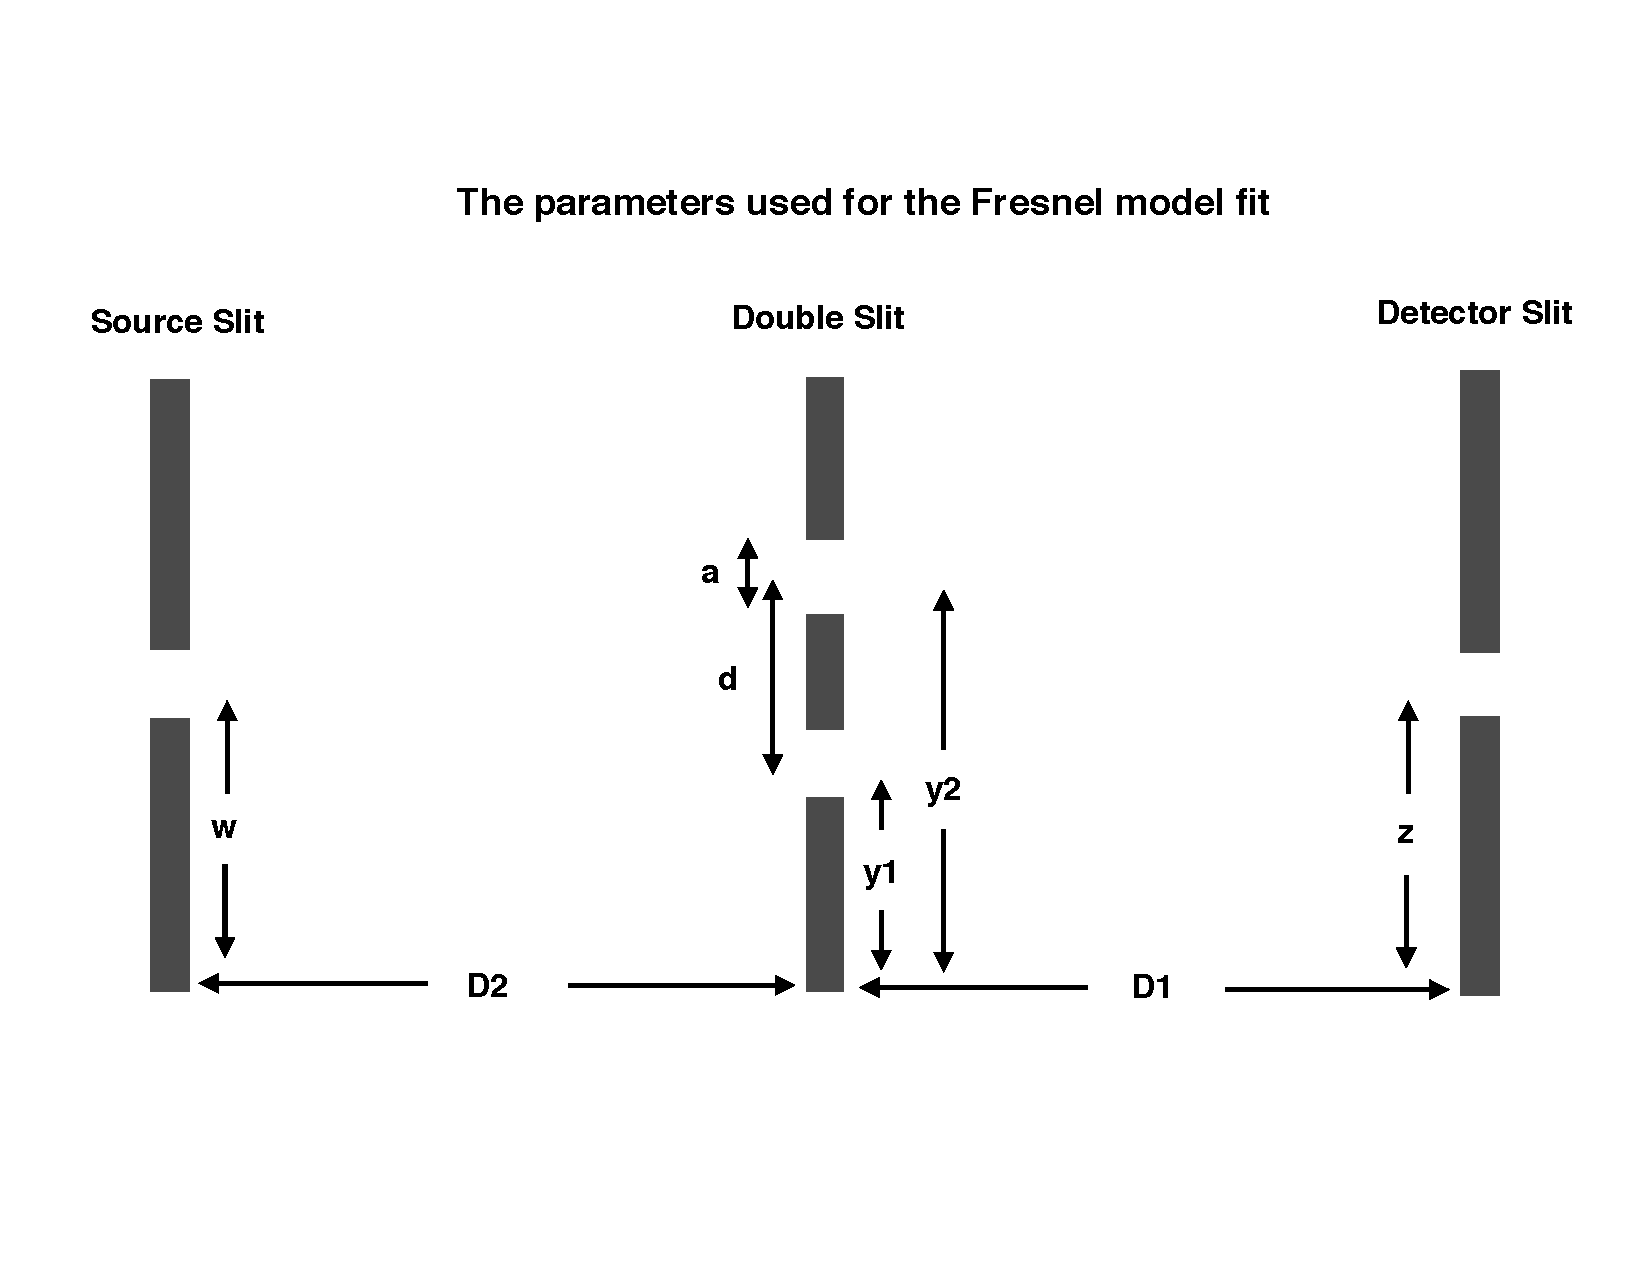
\includegraphics[width=6in]{fresnelsetup.pdf}
\caption{The set up of our double slit experiment showing the variables used for the Fresnel model fit. $D_1$ and $D_2$ are the distance from the source slit to the double slit and from the double slit to the detector slit respectively. $w$ is the displacement of the source slit from the light source. Since we aligned our source slit with our light source $w$ should be zero. $y_1$ and $y_2$ are the displacements of the double-slit slits from the center of source slit. These values are integrated to account for the width of each slit. $z$ was dependent on the location the detector slit and was related by $z = x - x_0$ to the x value of our data.}
\label{fresnelsetup}
\end{figure}

\begin{figure}[h!]
\centering
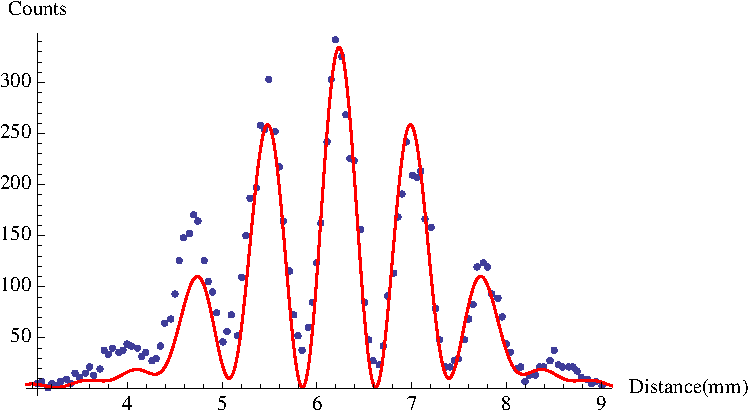
\includegraphics[width=6in]{doublefresnel1.pdf}
\caption{The fit to our first data set using the Fresnel model.}
\label{doublefresnel1}
\end{figure}

\begin{figure}[h!]
\centering
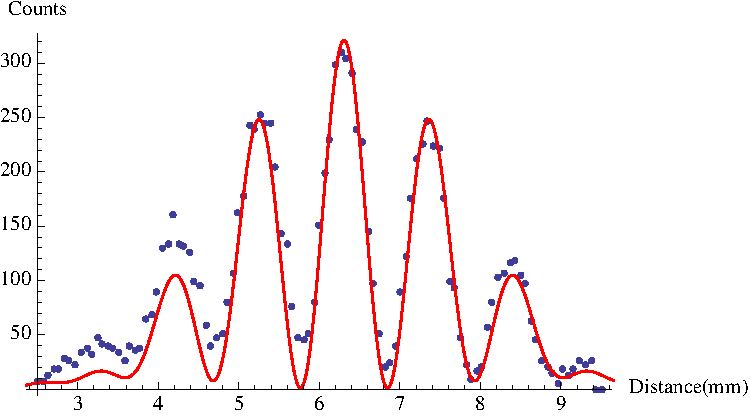
\includegraphics[width=6in]{doublefresnel2.pdf}
\caption{The fit to our second data set using the Fresnel model.}
\label{doublefresnel2}
\end{figure}

\begin{figure}[h!]
\centering
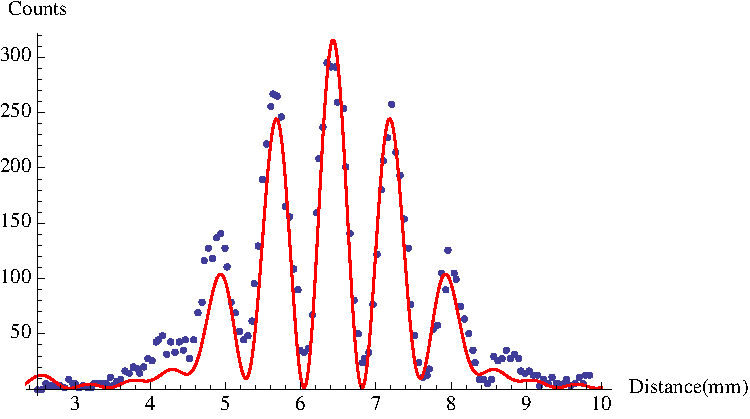
\includegraphics[width=6in]{doublefresnel3.pdf}
\caption{The fit to our third data set using the Fresnel model.}
\label{doublefresnel3}
\end{figure}


\begin{table}[h!]
\centering
\caption{The $\chi^2$ and reduced $\chi^2$ values for both the Fraunhofer and Fresnel fits for all three sets of data.}
\begin{ruledtabular}
\begin{tabular}{c c c c c}
Data Set & Fraunhofer $\chi^2$ & Fraunhofer Reduced $\chi^2$ & Fresnel $\chi^2$ & Fresnel Reduced $\chi^2$ \\
\hline	
1 & 510 &   73 & 374 &  53  \\
2 & 488 &   70 & 376 &  54  \\
3 & 856 & 122 & 857 & 122 \\

\end{tabular}
\end{ruledtabular}
\label{chisquared}
\end{table}

For the single slit data that we collected we were able to do a Fraunhofer model fit. The Fraunhofer model for a single slit gives the same function as Equation~\ref{fraunhofer} without the double slit diffraction. That leaves

\begin{equation}
\label{singlefraunhofer}
I(x) = I_0 \left(\frac{\sin\alpha}{\alpha}\right)^2
\end{equation}
 
 where $\alpha$ is once again

\begin{equation}
\label{alpha}
\alpha = \frac{a \pi \sin(\frac{x - x_0}{R})}{\lambda}
\end{equation}

Fitting Equation~\ref{singlefraunhofer} to our single slit data we got Figure~\ref{nearfraun} and Figure~\ref{farfraun}. As discussed above, the amplitude for our far slit data, Figure~\ref{farfraun}, is larger than expected most likely due to slit misalignment. Our near slit data, Figure~\ref{nearfraun}, agreed with our expectations for amplitude being one fourth the amplitude of the double slit fit.

\begin{figure}[h!]
\centering
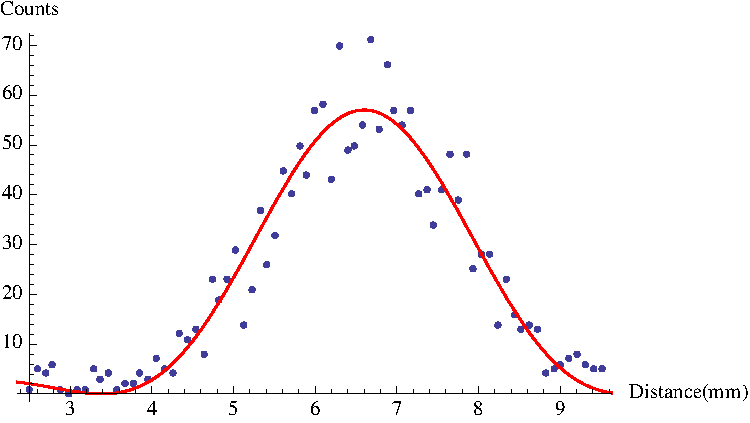
\includegraphics[width=6in]{nearfraun.pdf}
\caption{The fit to our near slit data using the Fraunhofer model. The amplitude meets expectations by being one fourth the amplitude of the double slit fit.}
\label{nearfraun}
\end{figure}

\begin{figure}[h!]
\centering
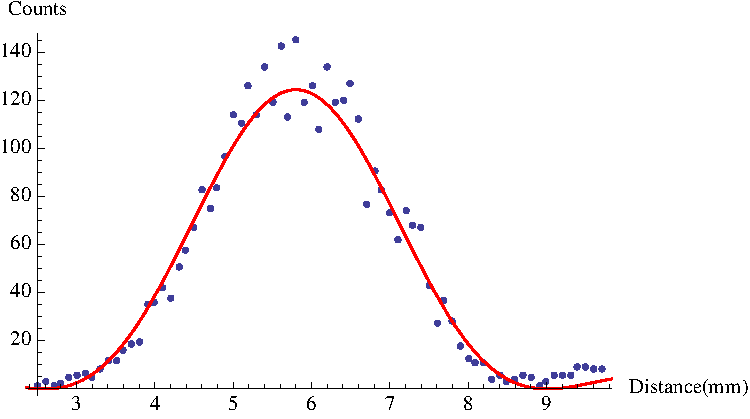
\includegraphics[width=6in]{farfraun.pdf}
\caption{The fit to our far slit data using the Fraunhofer model. The amplitude is much larger than expected due to slit misalignment.}
\label{farfraun}
\end{figure}

We attempted to fit our single slit data using the Fresnel model by only summing over a single slit, however the Mathematica file would not compile and we did not have time to problem solve the code error.


\section{Discussion}

The largest limiting factor in our experiment was the alignment of our slits. Aligning the slits was difficult because the light from the light bulb was too dim to see at the double slit. To align the slits we had to use the laser because it was bright enough to see all the way to the detection slit. However, this method is far from perfect because the laser was moveable and did not have the same positioning as the light bulb. So even if the slits were aligned using the laser, they would not necessarily be aligned when we switched to the light bulb.

To better align the slits we would have needed to take data with the light bulb, then realign the slits and take data again until the our data showed us the slits were aligned. Alignment could be seen when all the minima of the diffraction pattern reached zero. This method of fine alignment would have required more time than we had. Fine alignment would also have been difficult because we were adjusting the slits with our fingers so such small, precise movements would have been hard to achieve.

For future experiments we would suggest taking the time to make the fine adjustment necessary to ensure better alignment. And if possible use an apparatus that allows fine adjustments with something other than ones fingers.

Another potential difficulty was that our third data set had much higher $\chi^2$ and reduced $\chi^2$ values than than our first and second data sets. Further the $\chi^2$ and reduced $\chi^2$ values for third data set were same for both the Fraunhofer and Fresnel fits. Where as for our first and second data sets the $\chi^2$ and reduced $\chi^2$ values for the Fresnel fit was smaller than the $\chi^2$ and reduced $\chi^2$ values for the Fraunhofer fit. It appears that we had more noise around the edges of the diffraction pattern for our third data set than for the other two data sets. It is possible that this greater noise is reducing the accuracy of both our fits.

\section{Conclusion}

When shining coherent light through a pane with two closely spaced slits and onto a photo-detector, we saw a clear interference pattern, just like Young did, indicative of light acting as a wave. Of even greater significance, there is still a wave-like diffraction pattern observed even when there is only a single photon in the apparatus at a time. When analyzing this pattern, both the Fraunhofer and Fresnel model fits were relatively good (minus one particularly bad data set): 73, 70, and 122 for the Fraunhofer; 53, 54, and 122 for the Fresnel. The Fresnel model also fit better, indicating that the length of the chamber is small enough that it should be taken into account. Note as well that our parameters had a larger fluctuation when fitting the different data sets with the Fraunhofer model than with the Fresnel model. However, if this experiment is performed with a much longer chamber, the Fraunhofer model should begin to have a stronger $\chi^2$ correlation than the Fresnel.

\section{Appendix}

\begin{figure}[h!]
\centering
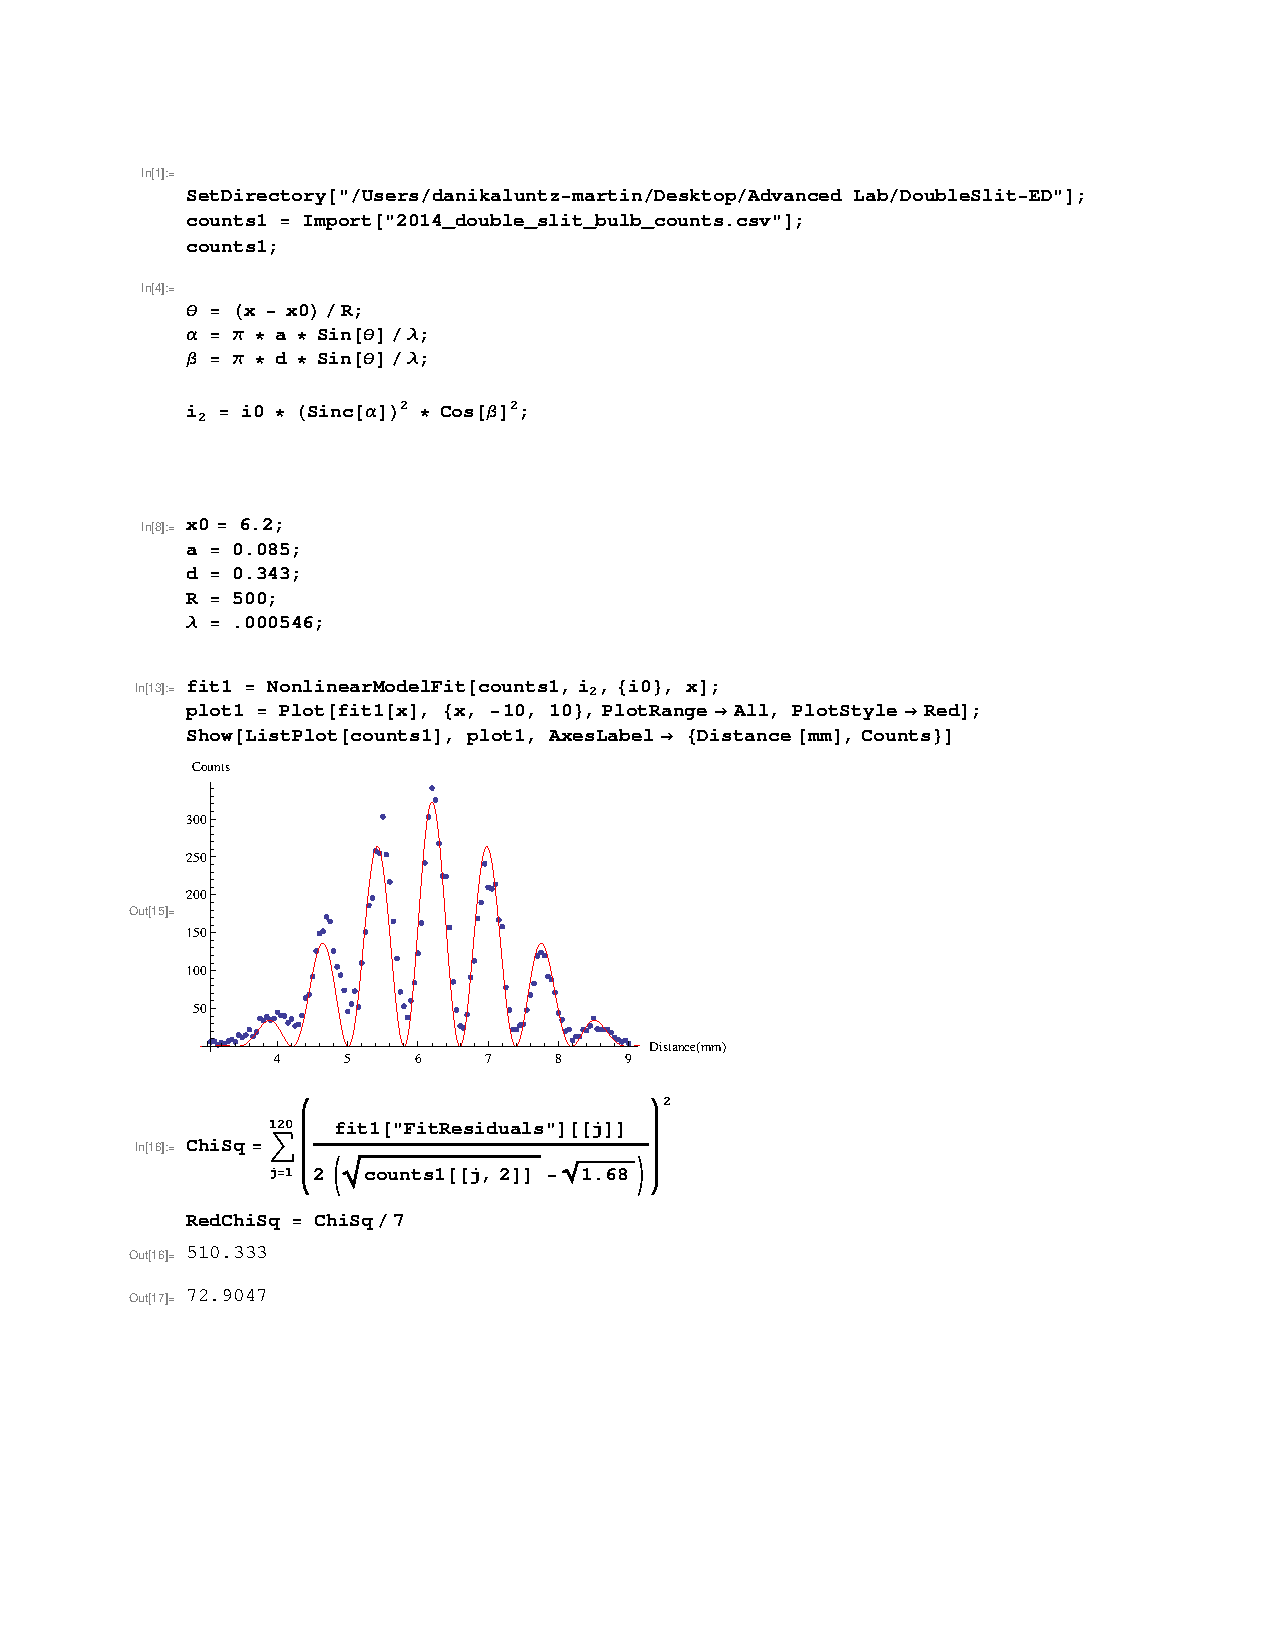
\includegraphics[width=6in]{DoubleSlitFraun1.pdf}
\caption{Mathematica code for the Fraunhofer model fit to our first double slit data set.}
\label{DoubleSlitFraun1}
\end{figure}

\begin{figure}[h!]
\centering
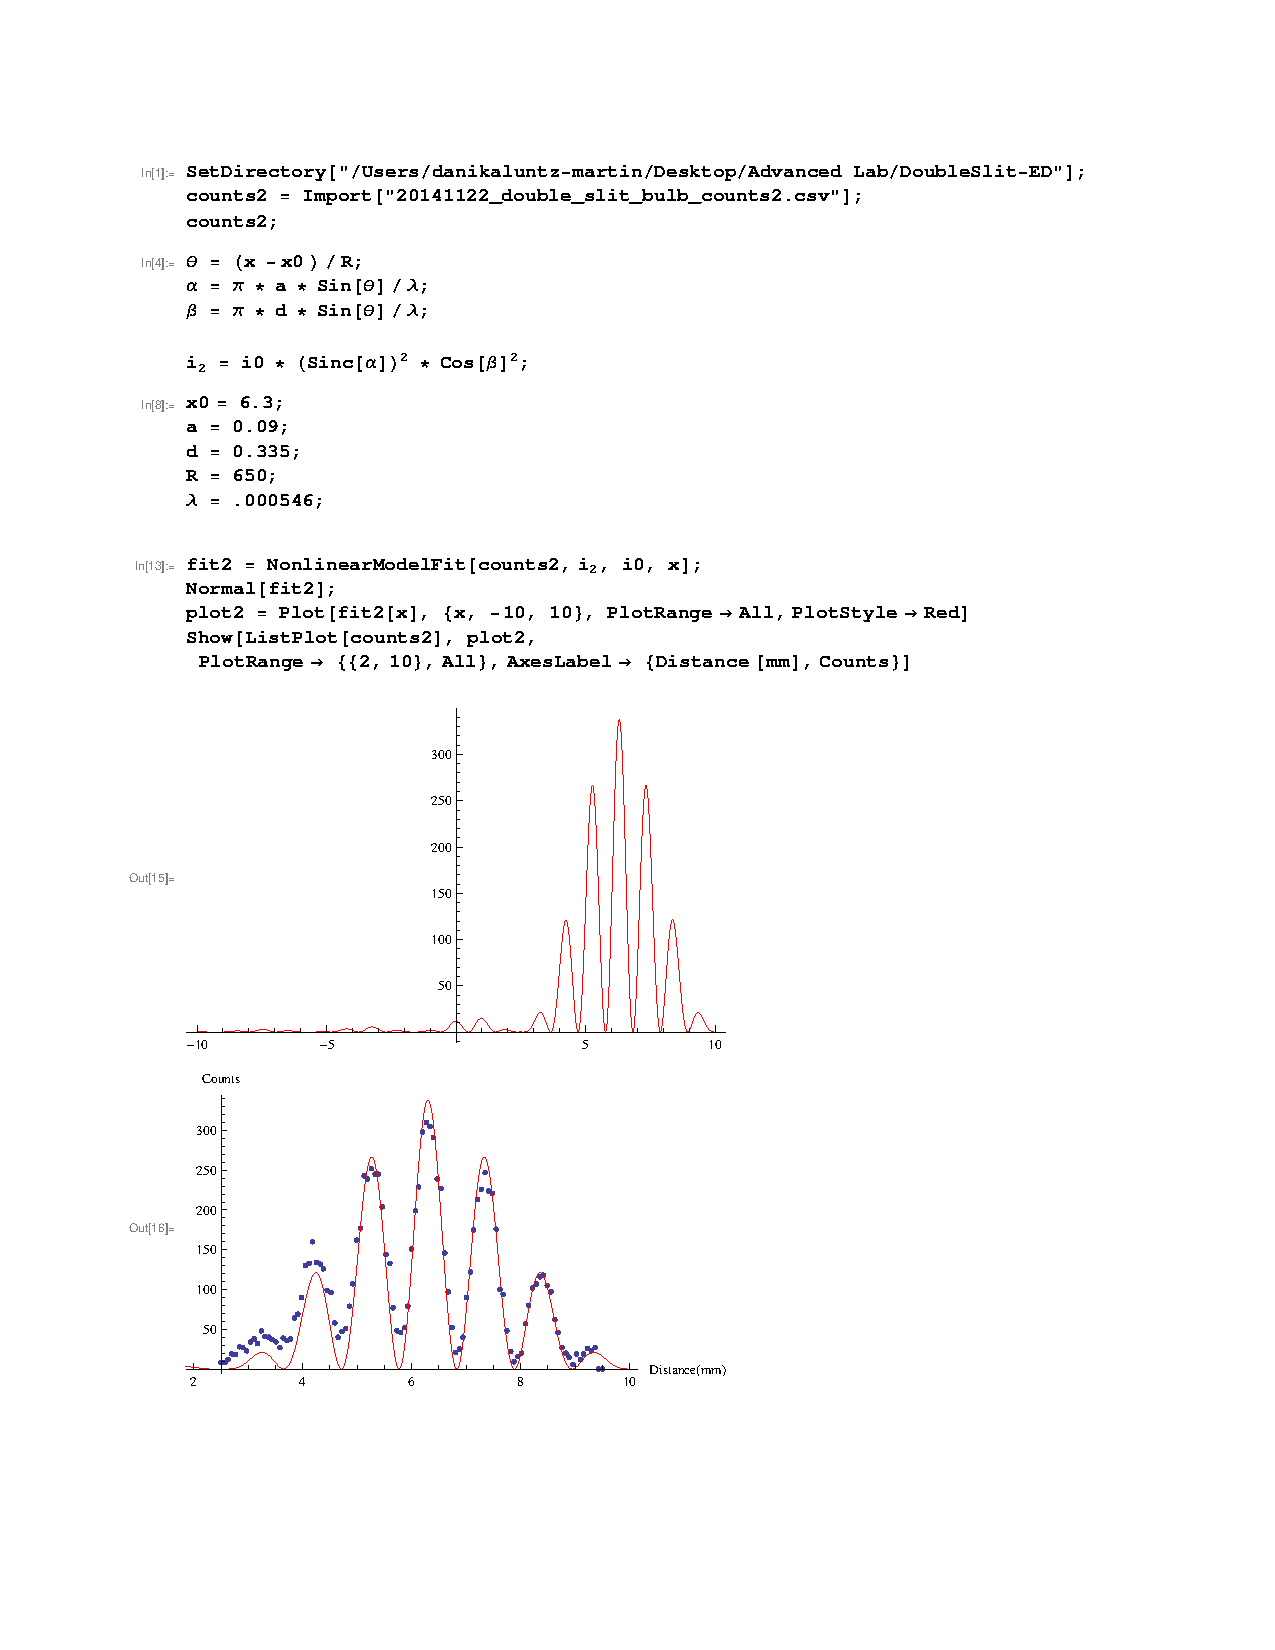
\includegraphics[width=6in]{DoubleSlitFraun2.pdf}
\caption{Mathematica code for the Fraunhofer model fit to our second double slit data set.}
\label{DoubleSlitFraun2}
\end{figure}


\begin{figure}[h!]
\centering
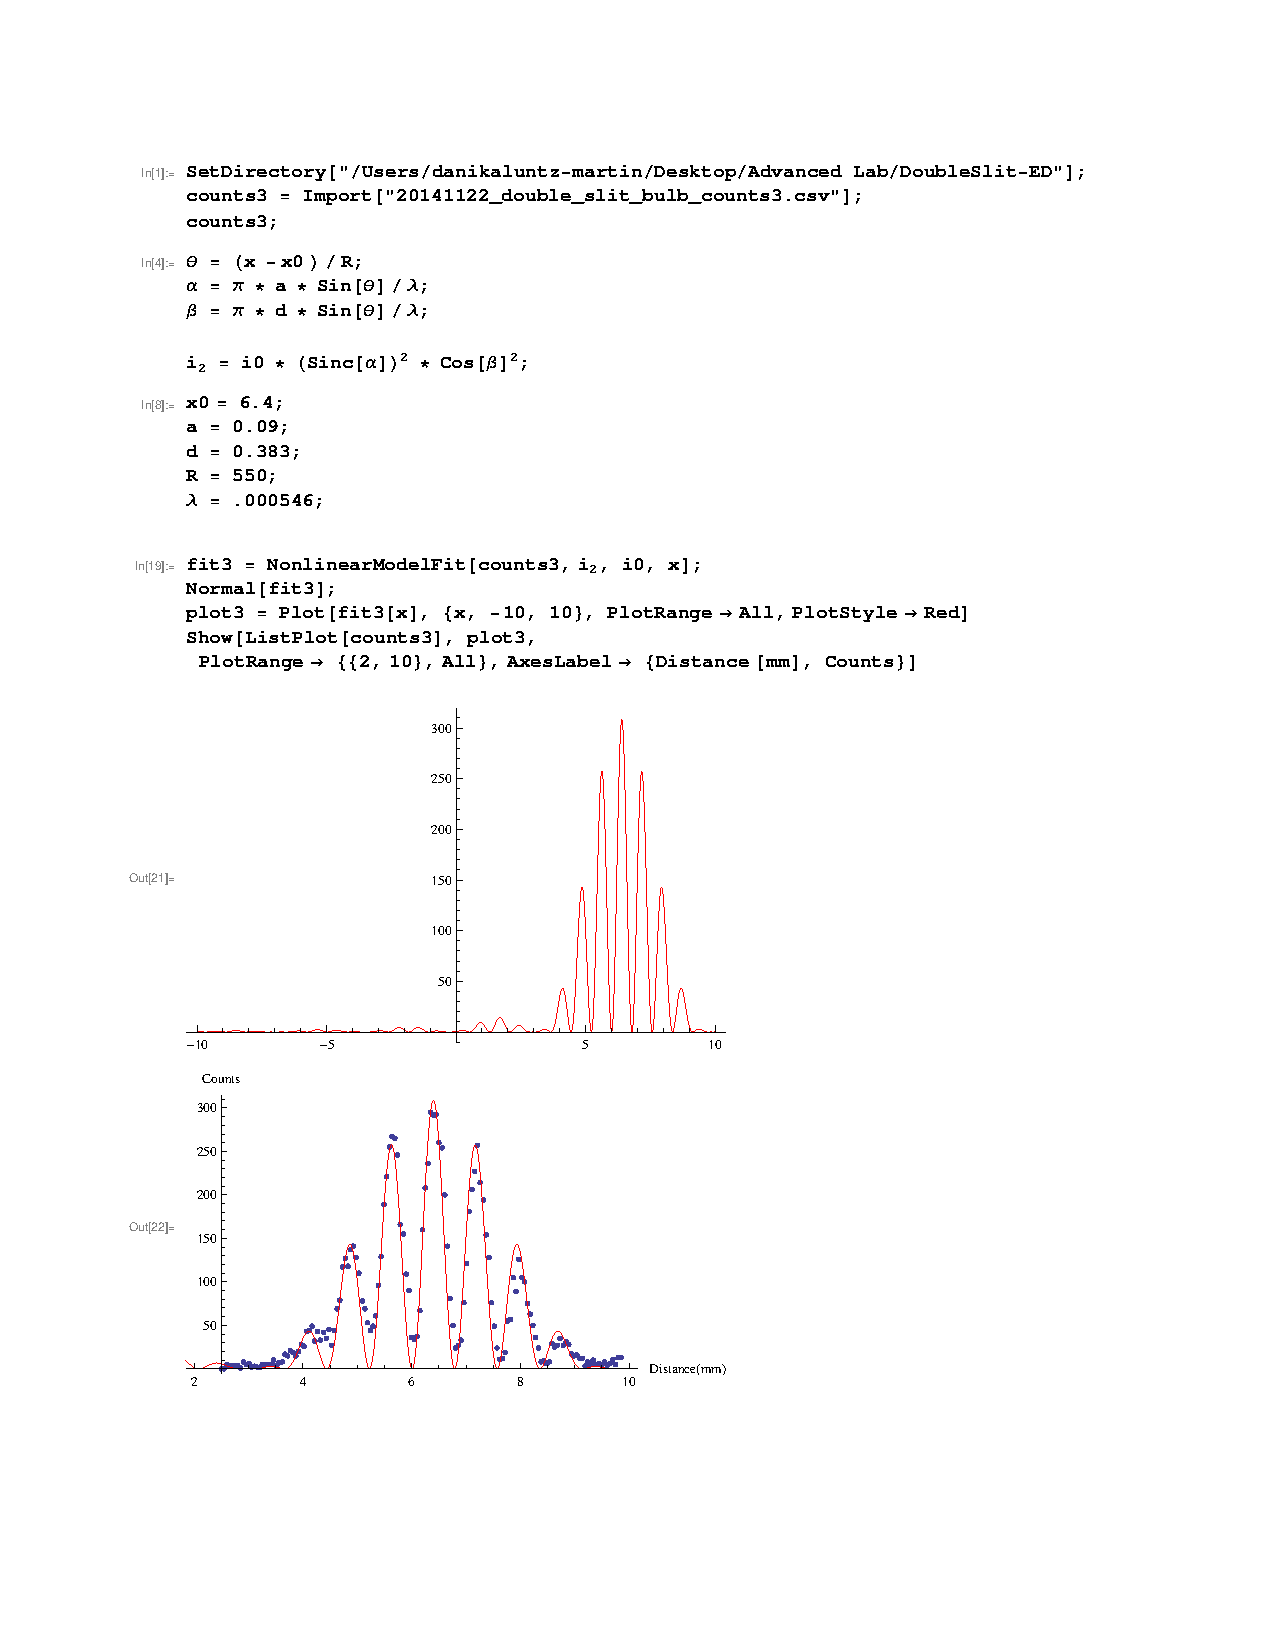
\includegraphics[width=6in]{DoubleSlitFraun3.pdf}
\caption{Mathematica code for the Fraunhofer model fit to our third double slit data set.}
\label{DoubleSlitFraun3}
\end{figure}

\begin{figure}[h!]
\centering
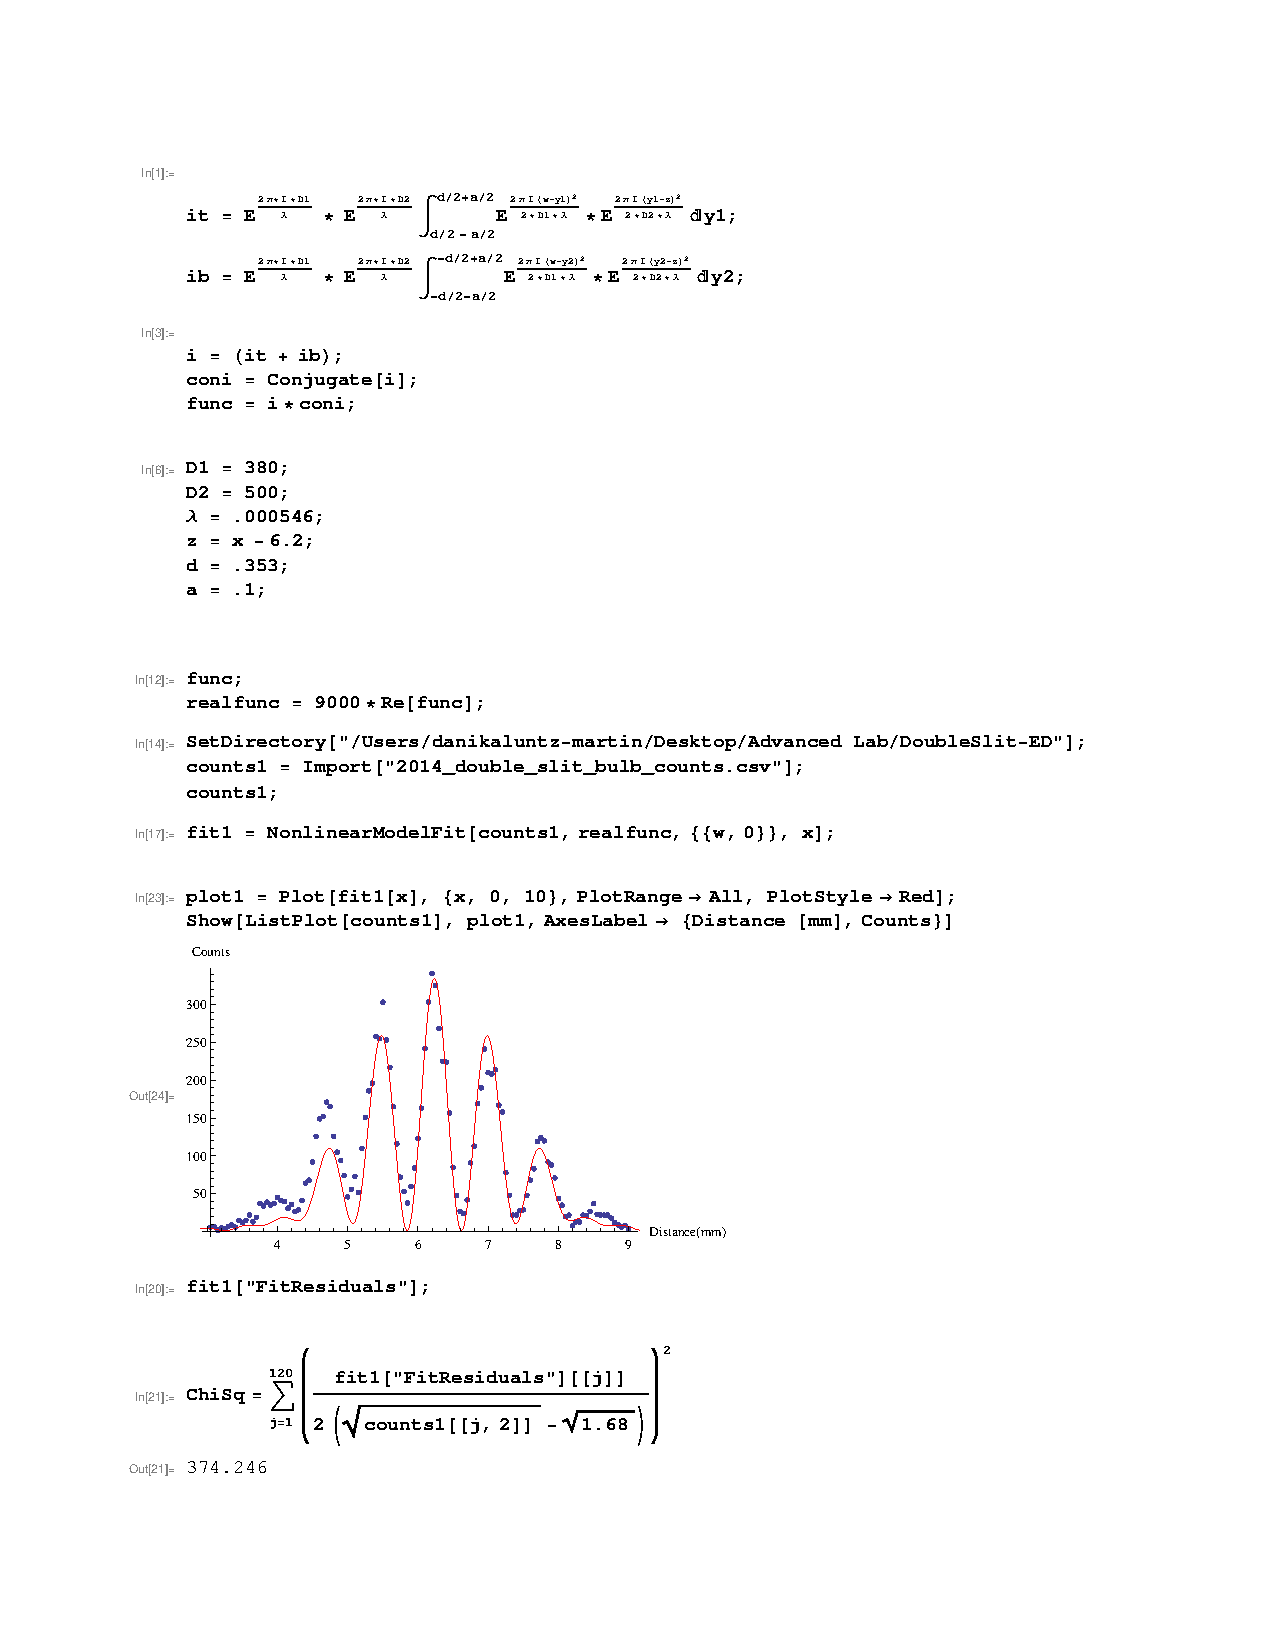
\includegraphics[width=6in]{DoubleSlitFresnel1.pdf}
\caption{Mathematica code for the Fresnel model fit to our first double slit data set.}
\label{DoubleSlitFresnel1}
\end{figure}

\begin{figure}[h!]
\centering
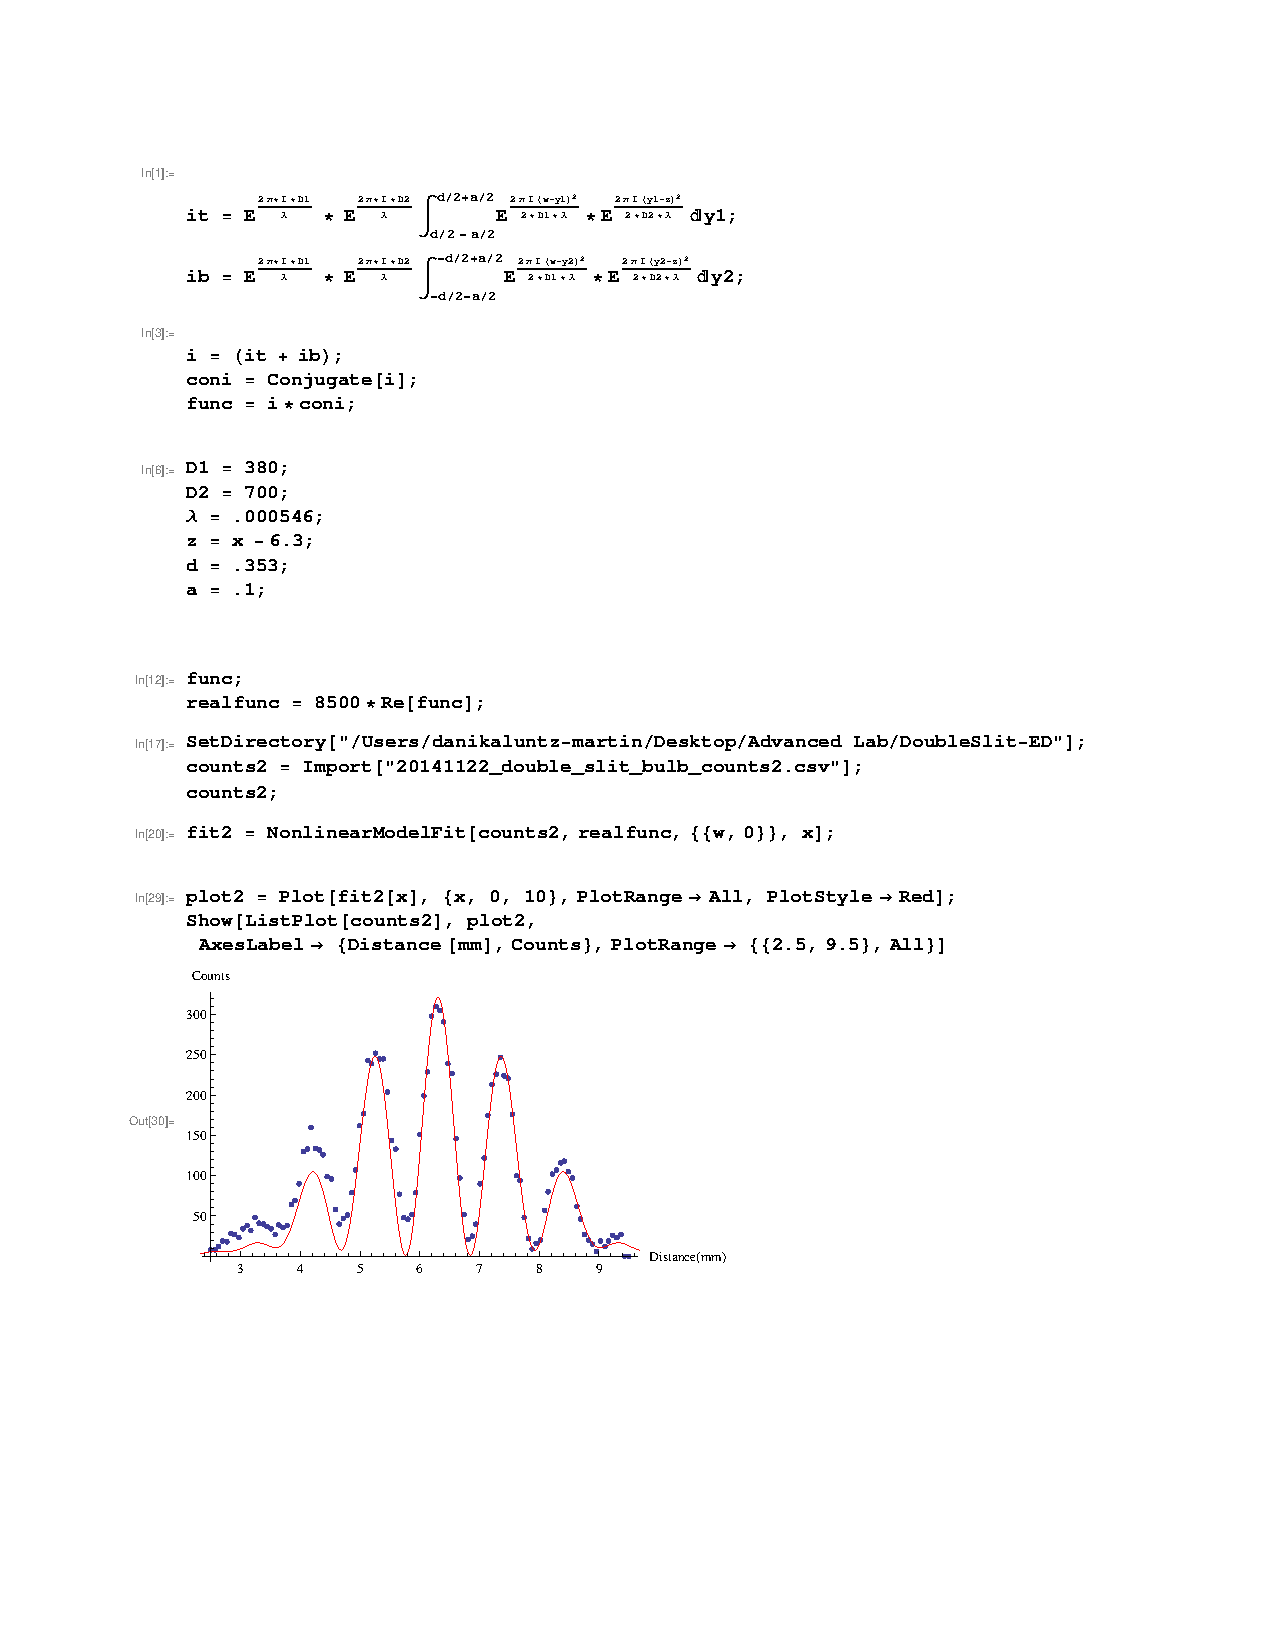
\includegraphics[width=6in]{DoubleSlitFresnel2.pdf}
\caption{Mathematica code for the Fresnel model fit to our second double slit data set.}
\label{DoubleSlitFresnel2}
\end{figure}

\begin{figure}[h!]
\centering
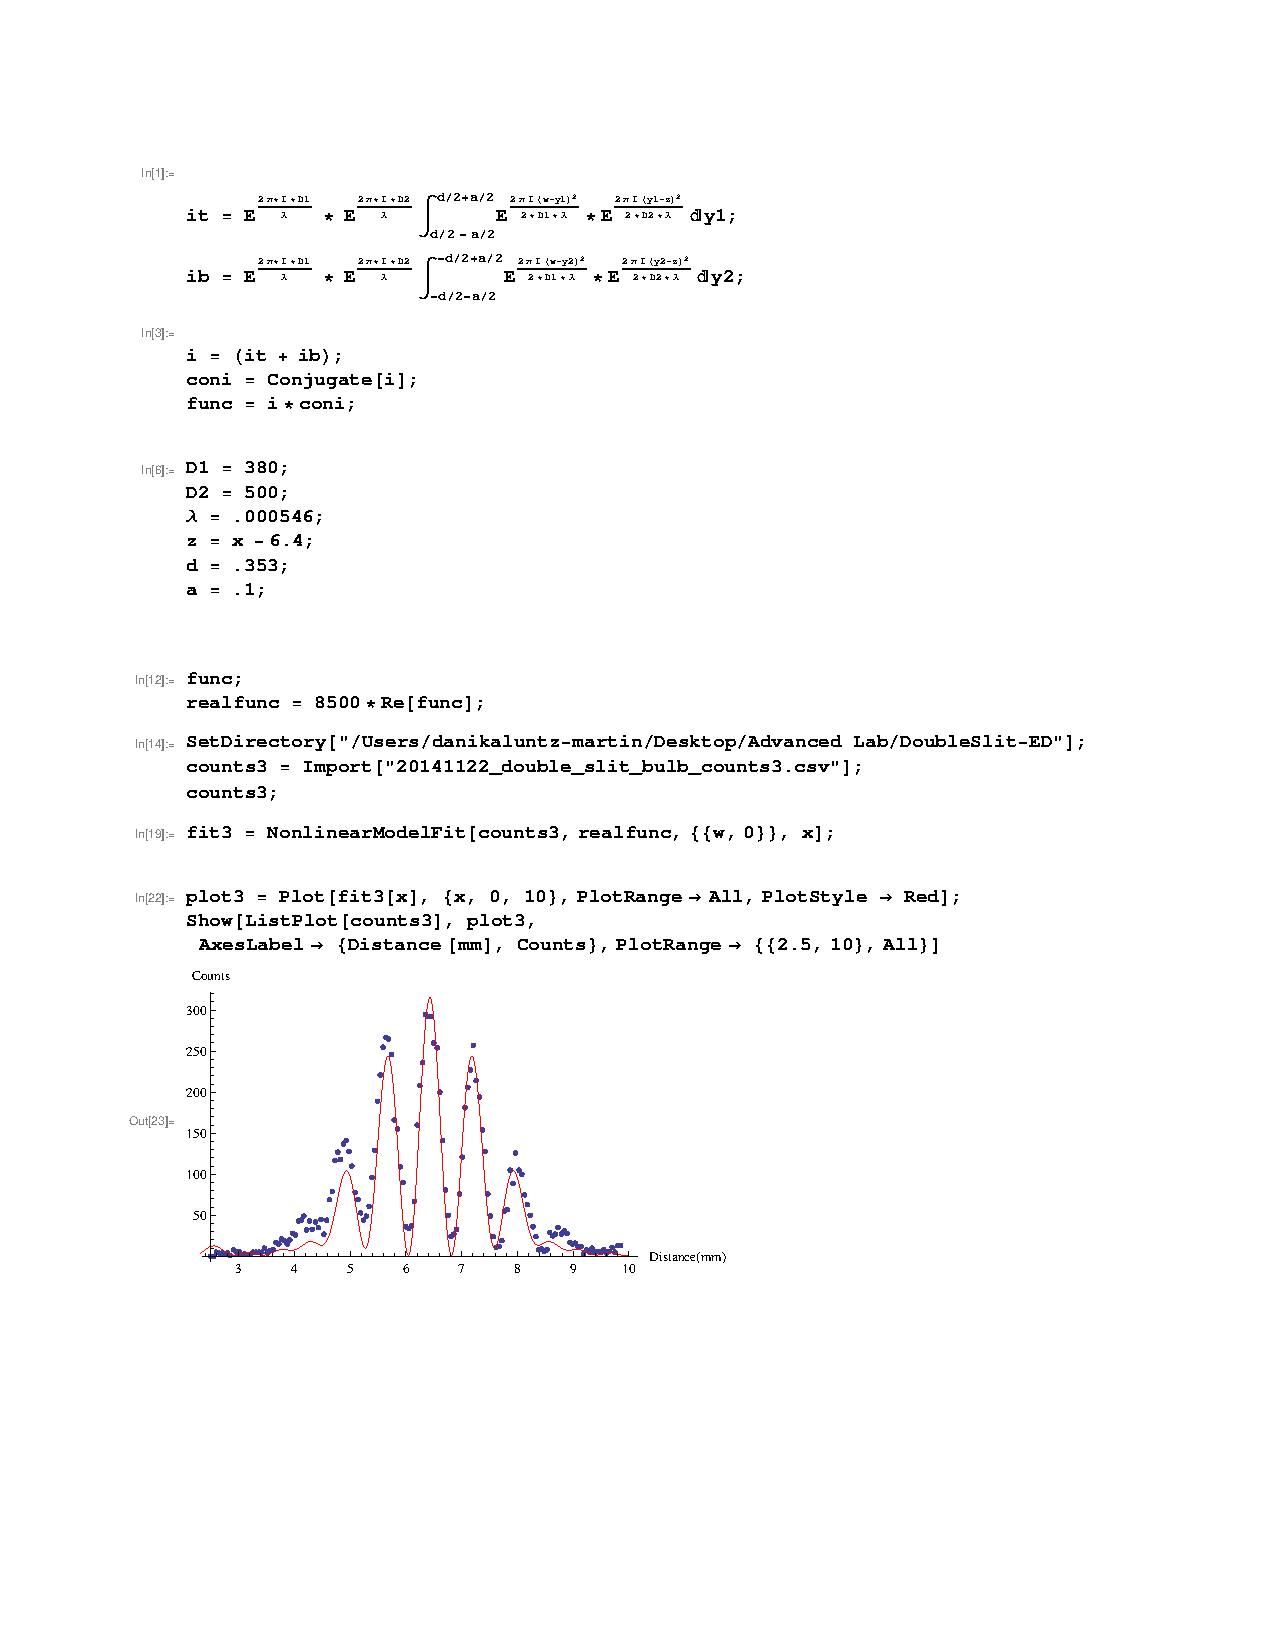
\includegraphics[width=6in]{DoubleSlitFresnel3.pdf}
\caption{Mathematica code for the Fresnel model fit to our third double slit data set.}
\label{DoubleSlitFresnel3}
\end{figure}

\begin{figure}[h!]
\centering
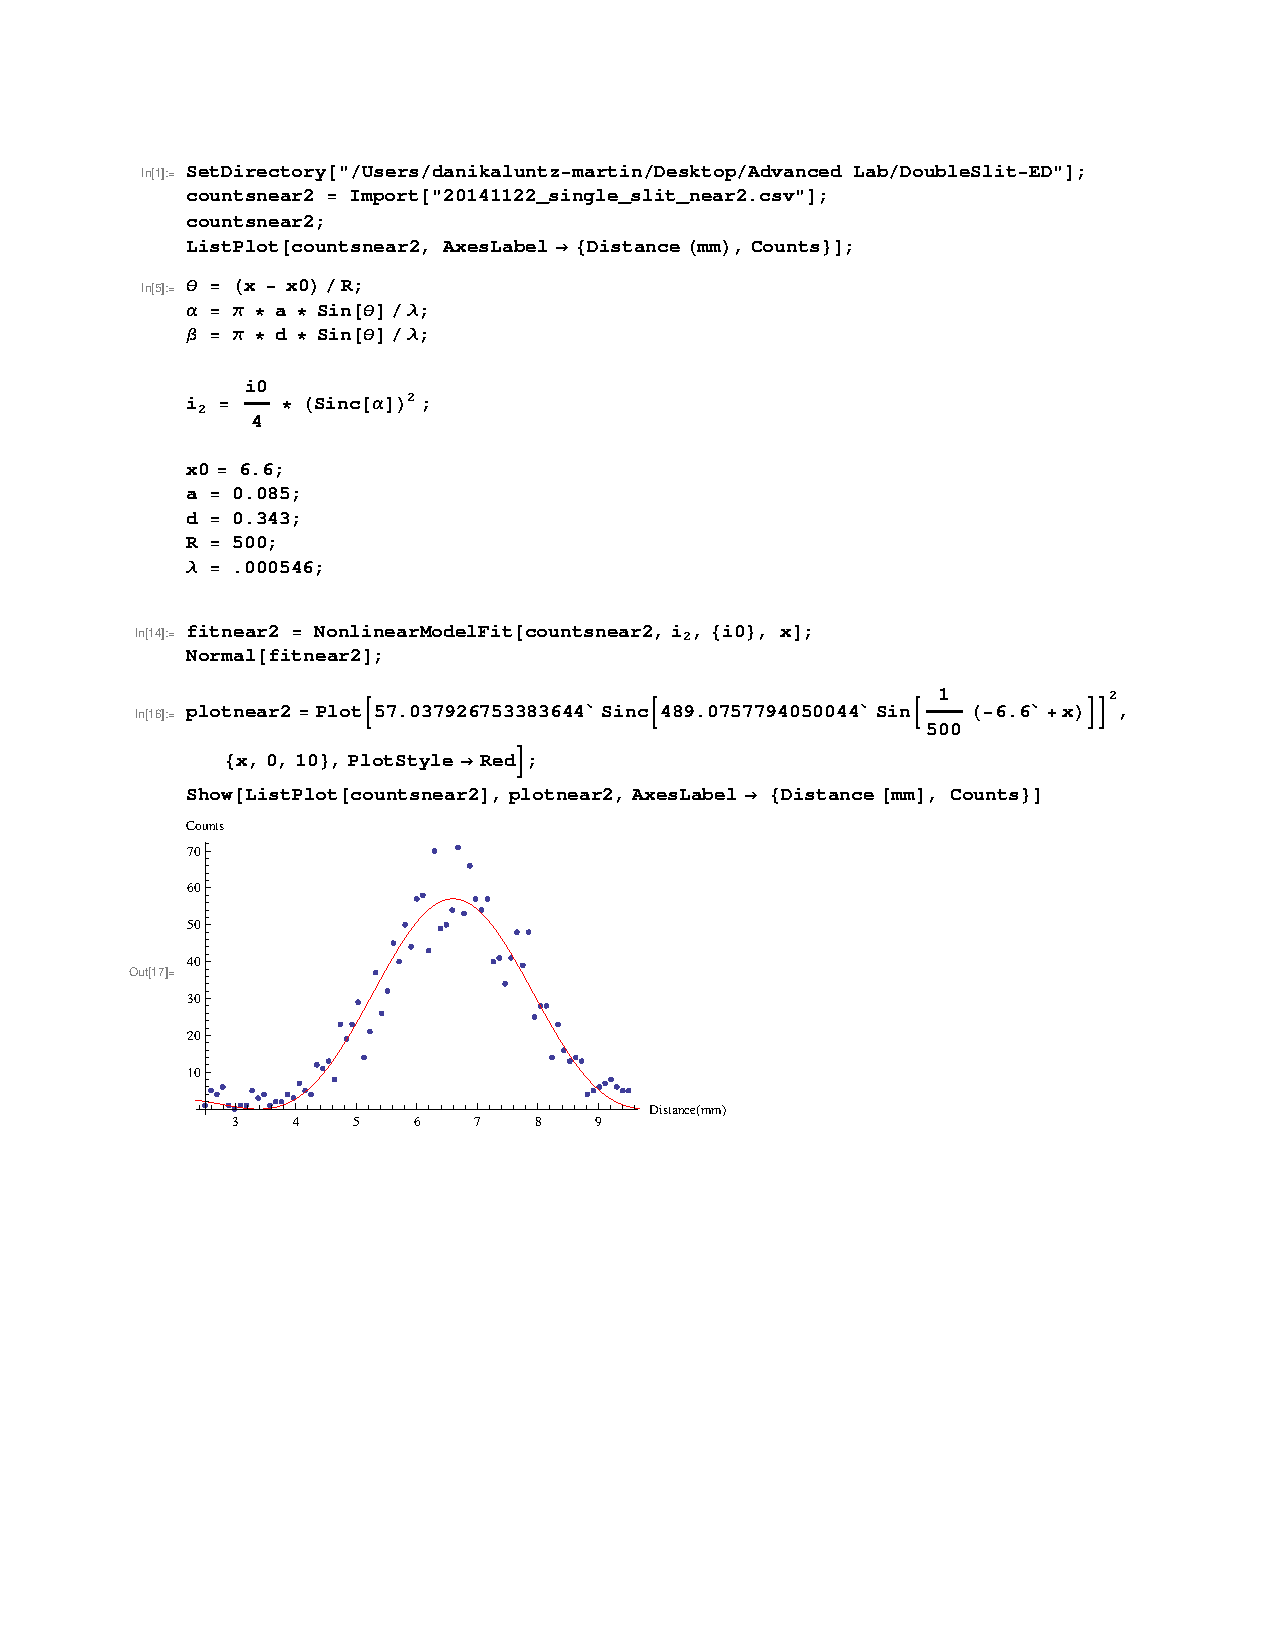
\includegraphics[width=6in]{SingleNearFraun.pdf}
\caption{Mathematica code for the Fraunhofer model fit to our near single slit data set.}
\label{SingleNearFraun}
\end{figure}

\begin{figure}[h!]
\centering
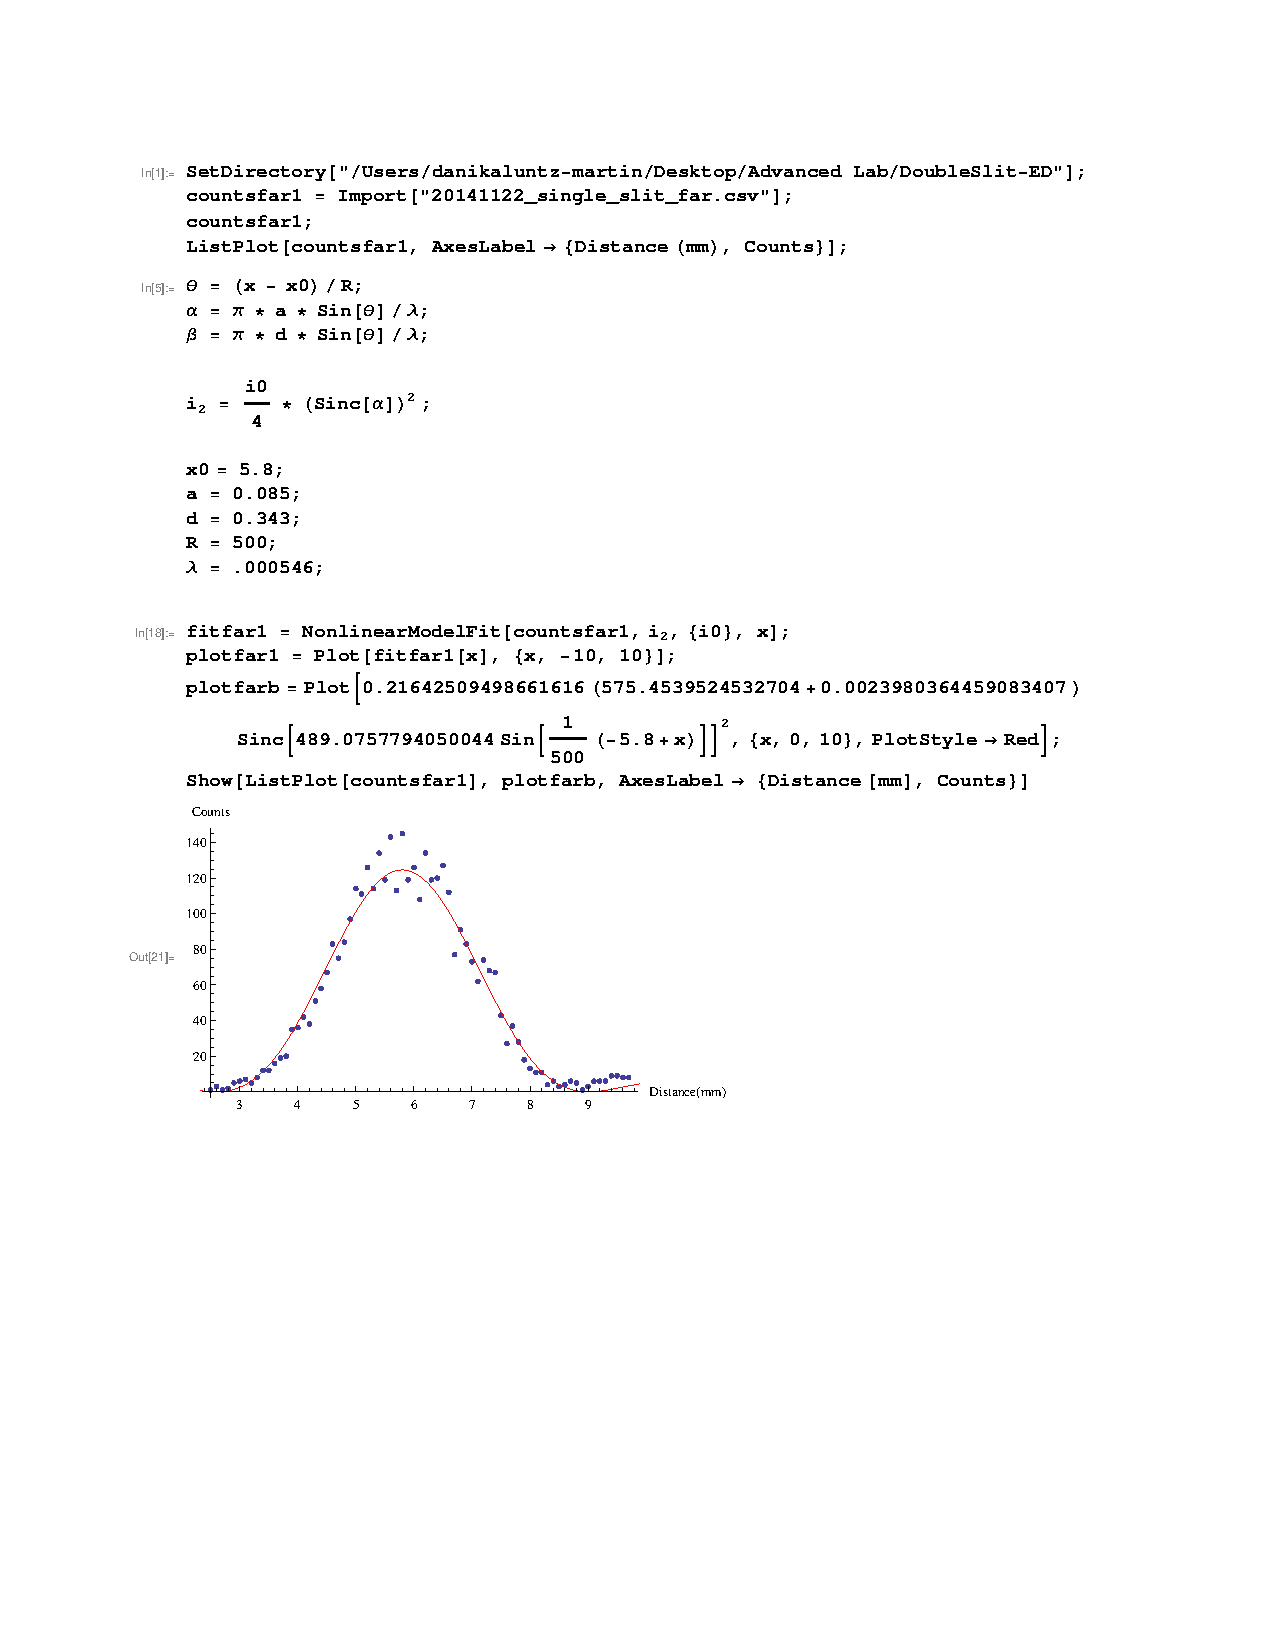
\includegraphics[width=6in]{SingleFarFraun.pdf}
\caption{Mathematica code for the Fraunhofer model fit to our far single slit data set.}
\label{SingleFarFraun}
\end{figure}

\newpage
\begin{thebibliography}{3}

\bibitem{studyphysics} Clintberg, Bryan. "Mr. Clintberg's Studyphysics!," 12/17/2014 \url{http://www.studyphysics.ca/newnotes/20/unit04_light/chp1719_light/lesson58.htm}

\bibitem{Wolfram} Weisstein, Eric. "Eric Weisstein's World of Physics," 12/17/2014. \url{http://scienceworld.wolfram.com/physics}

\bibitem{teachspin} Jonathan F. Reichert, \textit{TeachSpin Instruction Manuals: Two-Slit Interference, One Photon at a Time (TWS1 - B), Pulse Counter / Interval Timer (PCIT1)} Rev. 1.0, (2013)

\end{thebibliography}
\end{document}
